\documentclass{article}
\usepackage{xeCJK}
% if you need to pass options to natbib, use, e.g.:
%\PassOptionsToPackage{numbers, compress}{natbib}
% before loading nips_2017
%
% to avoid loading the natbib package, add option nonatbib:
% \usepackage[nonatbib]{nips_2017}

\usepackage[final]{nips_2017}

% to compile a camera-ready version, add the [final] option, e.g.:
% \usepackage[final]{nips_2017}

\usepackage[utf8]{inputenc} % allow utf-8 input
\usepackage[T1]{fontenc}    % use 8-bit T1 fonts
\usepackage{hyperref}       % hyperlinks
\usepackage{url}            % simple URL typesetting
\usepackage{booktabs}       % professional-quality tables
\usepackage{amsfonts}       % blackboard math symbols
\usepackage{nicefrac}       % compact symbols for 1/2, etc.
\usepackage{microtype}      % microtypography
\usepackage{bm}             % bold in math
\usepackage{graphicx}       % images
\usepackage{algorithm}      % algorithm
\usepackage[noend]{algpseudocode} % algorithm
\usepackage{caption}        % captionof
\usepackage{array}          % thick column hline
\usepackage{booktabs}       % table style
\usepackage{pbox}           % table line break
\usepackage{subcaption}     % multiple figures
\usepackage{listings}
\usepackage{xcolor}
\usepackage{tikz}
\usepackage{amsmath}
\definecolor{mygreen}{rgb}{0,0.6,0}
\definecolor{mygray}{rgb}{0.5,0.5,0.5}
\definecolor{mymauve}{rgb}{0.58,0,0.82}
\definecolor{codeBkg}{rgb}{0.85,0.85,0.85}

\lstset{ 
	backgroundcolor=\color{codeBkg},   % choose the background color; you must add \usepackage{color} or \usepackage{xcolor}; should come as last argument
	basicstyle=\footnotesize,        % the size of the fonts that are used for the code
	breakatwhitespace=false,         % sets if automatic breaks should only happen at whitespace
	breaklines=true,                 % sets automatic line breaking
	captionpos=b,                    % sets the caption-position to bottom
	commentstyle=\color{mygreen},    % comment style
	deletekeywords={...},            % if you want to delete keywords from the given language
	escapeinside={\%*}{*)},          % if you want to add LaTeX within your code
	extendedchars=true,              % lets you use non-ASCII characters; for 8-bits encodings only, does not work with UTF-8
	frame=no,	                   % adds a frame around the code
	keepspaces=true,                 % keeps spaces in text, useful for keeping indentation of code (possibly needs columns=flexible)
	keywordstyle=\color{blue},       % keyword style
	language=Octave,                 % the language of the code
	morekeywords={*,...},            % if you want to add more keywords to the set
	numbers=left,                    % where to put the line-numbers; possible values are (none, left, right)
	numbersep=5pt,                   % how far the line-numbers are from the code
	numberstyle=\tiny\color{mygray}, % the style that is used for the line-numbers
	rulecolor=\color{black},         % if not set, the frame-color may be changed on line-breaks within not-black text (e.g. comments (green here))
	showspaces=false,                % show spaces everywhere adding particular underscores; it overrides 'showstringspaces'
	showstringspaces=false,          % underline spaces within strings only
	showtabs=false,                  % show tabs within strings adding particular underscores
	stepnumber=1,                    % the step between two line-numbers. If it's 1, each line will be numbered
	stringstyle=\color{mymauve},     % string literal style
	tabsize=4,	                   % sets default tabsize to 2 spaces
	title=\lstname                   % show the filename of files included with \lstinputlisting; also try caption instead of title
}

\title{量化交易平台开发手册}

\hypersetup{
    colorlinks = true,
}
\makeatletter
\def\BState{\State\hskip-\ALG@thistlm}
\makeatother
\floatname{algorithm}{Procedure}
\renewcommand{\algorithmicrequire}{\textbf{Input:}}
\renewcommand{\algorithmicensure}{\textbf{Output:}}

\newcolumntype{?}{!{\vrule width 3pt}}

\author{
  闫涛 \\
  %% examples of more authors
  %% \And
  %% Nicholas Frosst \\
  %% Affiliation \\
  %% Address \\
  %% \texttt{email} \\
  %% \AND
  %% Geoffrey E. Hinton \\
  阿尔山金融科技有限公司\\
  北京 \\
  \texttt{\{yt7589\}@qq.com} \\
  %% Affiliation \\
  %% Address \\
  %% \texttt{email} \\
  %% \And
  %% Coauthor \\
  %% Affiliation \\
  %% Address \\
  %% \texttt{email} \\
  %% \And
  %% Coauthor \\
  %% Affiliation \\
  %% Address \\
  %% \texttt{email} \\
}
\date{March 2019}

% \usepackage{natbib}
% \usepackage{graphicx}

\begin{document}

\maketitle
\begin{abstract}
基于tushare.org开放数据集,构建本地量化交易开发平台。
\end{abstract}
\section{概述}
\subsection{环境搭建}
创建开源项目,项目网址:https://github.com/yt7589/aqp ,本地环境为:d:/awork/aftdc/incubate/aqp,虚拟环境激活:d:/aadesk/dev/python/quant/Script/activate ,这个是通过python -m venv quant来创建的虚拟环境。
\subsection{整体架构}
app\_main.py:程序主入口; \newline
app\_registry.py:管理程序中所有全局性配置和变量;\newline
controller目录:所有业务逻辑实现类;\newline
model目录:所有数据库操作类;\newline
\subsection{数据服务商}
我们采用的是tushare.pro提供的数据服务:https://tushare.pro 。
\subsection{Python单元测试}
我们采用类似测试驱动开发方式,主要功能都要有单元测试,因此需要使用单元测试框架。我们采用unittest单元测试框架,
下面我们以一个具体的例子为例,来说明怎样使用单元测试框架。我们来看怎样从t\_account\_io表的某个账户中转出现金
的10\%。我们首先建立test目录,存放所有单元测试用例。\newline
首先建立测试用例目录,其名称为tdd,注意:不要叫test目录,这个目录会有问题。\newline
我们建立账户流水控制器类controller/c\_account\_io.py,如下所示:
\lstset{language=PYTHON, caption={账户流水类}, label={c000007}}
\begin{lstlisting}
class CAccountIo(object):
def __init__(self):
    self.name = 'CAccountIo'

@staticmethod
def withdraw(account_id, amount):
    '''
    从指定账户取出指定金额,增加资金转出金额记录,并更新用户现金资产
    '''
    print('CAccountIo.withdraw')

#股票预测:
#https://medium.com/m/global-identity?redirectUrl=https%3A%2F%2Ftowardsdatascience.com%2Faifortrading-2edd6fac689d
\end{lstlisting}
在测试目录下创建对应的测试类tdd/controller/t\_c\_account\_io.py,如下所示:
\lstset{language=PYTHON, caption={账户流水测试类}, label={c000008}}
\begin{lstlisting}
import unittest
from controller.c_account_io import CAccountIo

class TCAccountIo(unittest.TestCase):
    def test_withdraw(self):
        account_id = 1
        amount = 100
        CAccountIo.withdraw(account_id, amount)
        self.assertEqual('abc', 'abc')

if '__main__' == __name__:
    unittest.main()
\end{lstlisting}
测试入口类app\_test.py,如下所示:
\lstset{language=PYTHON, caption={单元测试入口类}, label={c000009}}
\begin{lstlisting}
from tdd.controller.t_c_account_io import TCAccountIo
\end{lstlisting}
运行单元测试用例命令为:
\lstset{language=BASH, caption={测试程序命令行执行}, label={c000010}}
\begin{lstlisting}
python -m unittest -v app_test.py
\end{lstlisting}
运行结果如下所示:
\begin{figure}[H]
	\caption{单元测试运行结果}
	\label{f000002}
	\centering
	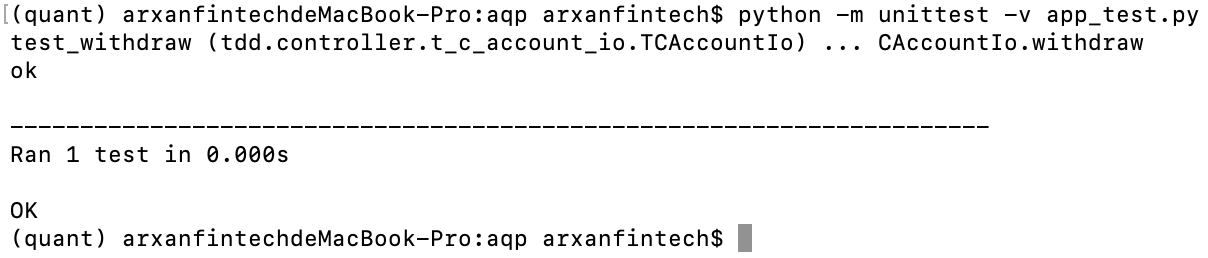
\includegraphics[height=3cm]{images/f000002}
\end{figure}
\subsection{Flask入门}
Flask框架目前已经超越Django,成为Python语言Web开发中最流行的框架。
\subsubsection{入门程序}
使用flask进行Web开发非常简单,因为实际应用中python只用于提供API接口,因此我们以API服务器为例:
\lstset{language=PYTHON, caption={Hello World级Flask程序}, label={c000011}}
\begin{lstlisting}
import json
from flask import Flask

app = Flask(__name__)

@app.route('/')
def hello_world():
    resp = {'code': 1}
    resp['result'] = {}
    resp['result']['userId'] = 101
    return json.dumps(resp)

app.run(port=5080, debug=True)
\end{lstlisting}
上述程序中,监听在5080端口,返回值为JSON格式。
\subsubsection{路径中的参数}
在很多情况下,我们需要将路径中的部分作为参数,具体处理方式如下所示:
\lstset{language=PYTHON, caption={处理path中的参数}, label={c000012}}
\begin{lstlisting}
@app.route('/user/<int:user_id>/<string:user_name>/<email>', methods=['GET'])
def process_path_params(user_id, user_name, email):
    resp = {'code': 1}
    resp['result'] = {}
    resp['result']['userId'] = user_id
    resp['result']['userName'] = user_name
    resp['result']['email'] = email
    return json.dumps(resp)
\end{lstlisting}
参数可以带类型说明也可以不带,同时分号两边不能有空格。methods可以为GET或POST。
\subsubsection{处理QueryString}
获取URL中的参数可以采用下面的方法:
\lstset{language=PYTHON, caption={获取URL中的参数}, label={c000013}}
\begin{lstlisting}
@app.route('/get_url_params/t1', methods=['GET'])
def get_url_params():
    resp = {'code': 1}
    resp['result'] = {}
    resp['result']['url'] = url_for('get_url_params')
    resp['result']['userId'] = request.args['userId']
    # args类型为ImmutableMultiDict
    params = request.args.to_dict()
    resp['result']['params'] = params
    return json.dumps(resp)
\end{lstlisting}
如上所示,url\_for可以打印出完整的URL路径,参数为路径中第一个分量。request.args为不可变字典,也可以将其转变为
普通字典。
\subsubsection{处理form}
当请求为POST时,参数是通过form来传递的,这时需要解析form中的参数:
\lstset{language=PYTHON, caption={获取URL中的参数}, label={c000013}}
\begin{lstlisting}
@app.route('/get_post_params/t2', methods=['POST'])
def get_post_params():
    resp = {'code': 1}
    resp['result'] = {}
    resp['result']['userName'] = request.form['userName']
    params = request.form.to_dict()
    return json.dumps(json)
\end{lstlisting}
\subsubsection{session处理}
略。
\subsubsection{cookie处理}
略。
\subsubsection{文件上传处理}
略。
\subsubsection{数据库连接池}





\section{数据处理}
数据处理包括从tushare.org网站获取数据,将其转化为量化平台所需的数据格式。
\subsection{获取沪深市场所有挂牌股票}
获取在沪深两市挂牌的所有股票的基本信息。
\subsubsection{接口定义}
获取股票基本信息接口为stock\_basic,其参数为:

\begin{table}[H]
\caption{stock\_basic接口输入参数说明}
\label{t000001}
\begin{tabular}{|c|c|c|c|} \hline
名称 & 类型 & 必选 & 描述 \\ \hline  
is\_hs & str & N & 是否沪深港通标的,N否 H沪股通 S深股通 \\ \hline
list\_status & str & N & 上市状态: L上市 D退市 P暂停上市 \\ \hline
exchange & str & N & 交易所:SSE上交所 SZSE深交所 HKEX港交所 \\ \hline
\end{tabular}
\end{table}

返回值为:
\begin{table}[H]
\caption{stock\_basic接口返回结果说明}
\label{t000002}
\begin{tabular}{|c|c|c|} \hline
名称 & 类型 & 描述 \\ \hline  
ts\_code & str & TS代码 \\ \hline
symbol & str & 股票代码 \\ \hline
name & str & 股票名称 \\ \hline
area & str & 所在地域 \\ \hline
industry & str & 所属行业 \\ \hline
fullname & str & 股票全称 \\ \hline
enname & str & 英文全称 \\ \hline
market & str & 市场类型 (主板/中小板/创业板) \\ \hline
exchange & str & 交易所代码 \\ \hline
curr\_type & str & 交易货币 \\ \hline
list\_status & str & 上市状态: L上市 D退市 P暂停上市 \\ \hline
list\_date & str & 上市日期 \\ \hline
delist\_date & str & 退市日期 \\ \hline
is\_hs & str & 是否沪深港通标的,N否 H沪股通 S深股通 \\ \hline
\end{tabular}
\end{table}


调用格式为:
\lstset{language=PYTHON, caption={获取股票基本信息}, label={c000001}}
\begin{lstlisting}
import tushare as ts
pro = ts.pro_api()
data = pro.stock_basic(exchange='', list_status='L', 
                    fields='ts_code,symbol,name,area,industry,list_date')
data = pro.query('stock_basic', exchange='', list_status='L', 
			fields='ts_code,symbol,name,area,industry,list_date')
\end{lstlisting}
见\ref{c000001}所示
结果示例:
\lstset{language=BASH, caption={获取股票基本信息结果示例}, label={c000002}}
\begin{lstlisting}
    ts_code     symbol     name     area industry    list_date
0     000001.SZ  000001  平安银行   深圳       银行  19910403
1     000002.SZ  000002   万科A   深圳     全国地产  19910129
2     000004.SZ  000004  国农科技   深圳     生物制药  19910114
3     000005.SZ  000005  世纪星源   深圳     房产服务  19901210
4     000006.SZ  000006  深振业A   深圳     区域地产  19920427
5     000007.SZ  000007   全新好   深圳     酒店餐饮  19920413
\end{lstlisting}

\subsubsection{区域信息}
如代码\ref{c000002}所示,地区是以字符串形式返回的。我们可能需要按地区来统计股票表现,因此需要将地区统计出来,放到单独的一个表中进行管理。
\paragraph{数据库设计}
数据库结构表结构如下所示:
\lstset{language=SQL, caption={地区表数据结构}, label={c000003}}
\begin{lstlisting}
create table t_area(
	area_id int primary key auto_increment,
	area_name varchar(200)
);
\end{lstlisting}
\paragraph{信息处理}
当我们读到返回结果的一行时,我们取出地区信息,然后查询t\_area表中是否包含该地区,如果包含则返回对应的area\_id,否则将该地区添加到t\_area表中,并返回其area\_id。
\subsubsection{行业信息}
\paragraph{数据库设计}
\paragraph{信息处理}
\subsubsection{股票信息}
\paragraph{接口定义}
\paragraph{获取并处理数据}
\subsection{获取日线行情数据}
\section{量化模型}
\subsection{时间序列分析}
\section{回测系统}
\subsection{数据库系统设计}
客户是自然人,用t\_customer表示。客户加上账户再加上量化策略,形成我们系统的用户,用t\_user来表示。
账户中具有现金资产和股票资产。
账户具有资金的入和出,有股票的买入和卖出。
用户持有一些股票,可以对股票进行买卖。
用户可以买入和卖出指定数量股票,与账户资金变动相关联
股票参数表:买入费率、印花税;卖出费率、印花税等,计入交易成本中。
\subsubsection{ER图}
\begin{figure}[H]
	\caption{数据库表ER图}
	\label{f000001}
	\centering
	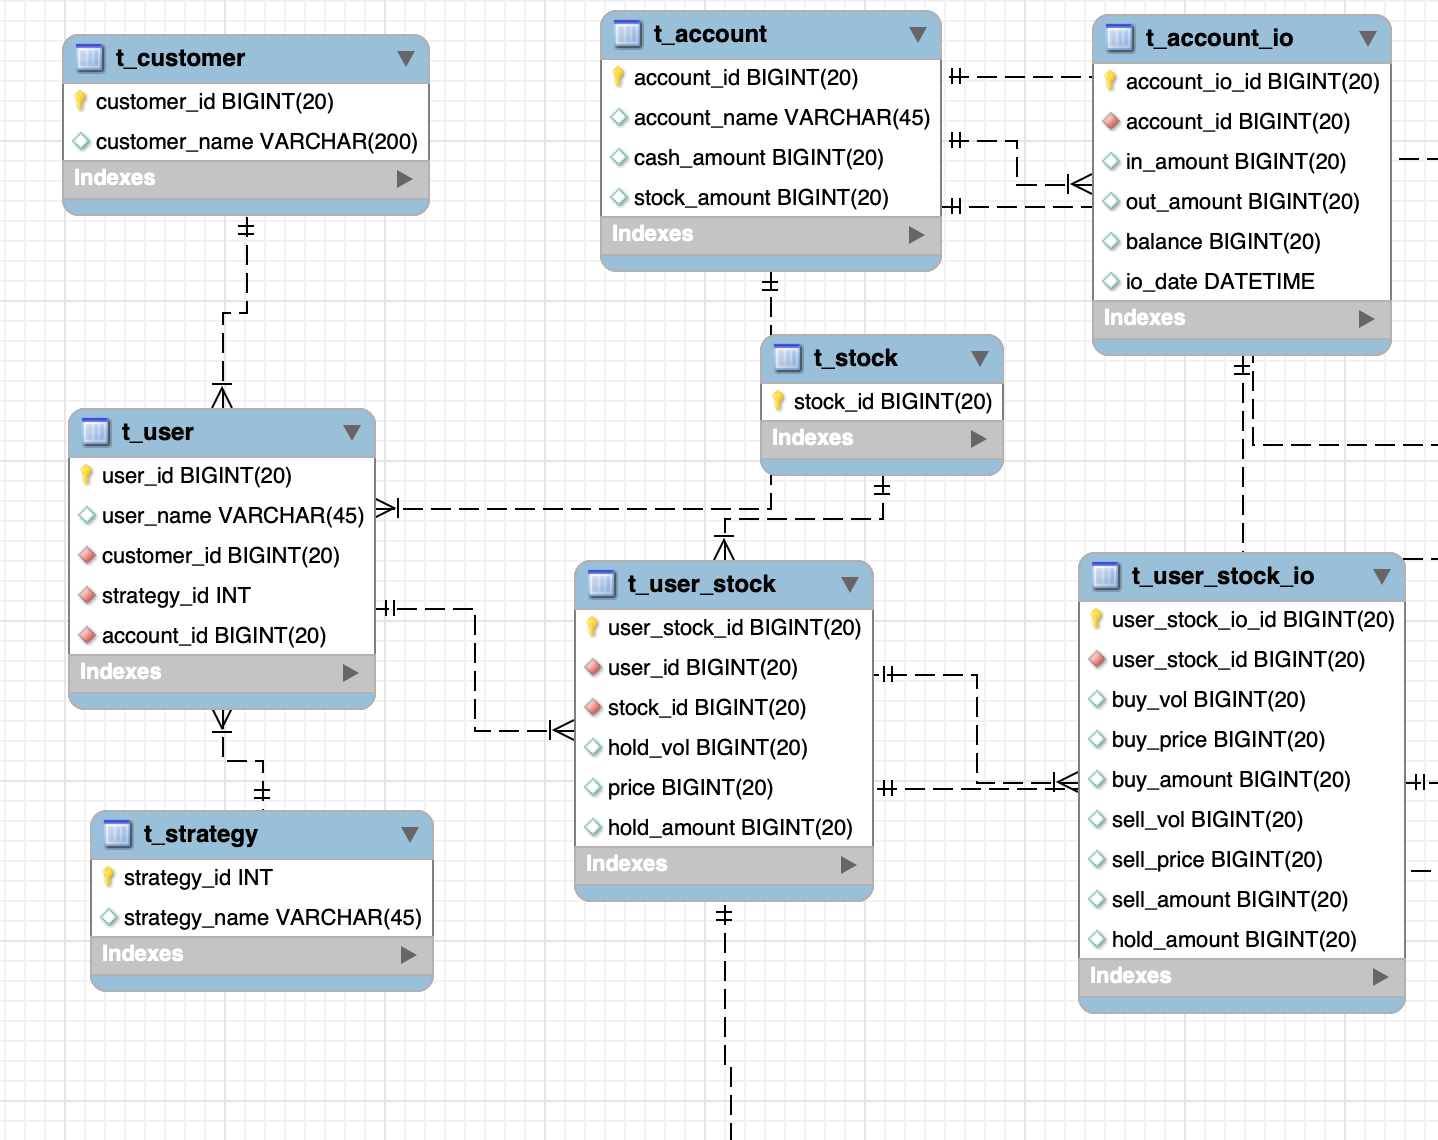
\includegraphics[height=10cm]{images/f000001}
\end{figure}
\subsubsection{客户表}
表示自然人客户,结构如下所示:
\begin{table}[H]
    \caption{客户表(t\_custome)}
    \label{t000001}
    \begin{tabular}{|p{2cm}|p{3cm}|p{2cm}|p{5cm}|} \hline
        字段 & 名称 & 类型 & 描述 \\ \hline 
        customer\_id & 客户编号 & bigint & 主键且自增长 \\ \hline
        customer\_name & 客户姓名 & varchar & 真实姓名 \\ \hline
    \end{tabular}
\end{table}
\subsubsection{策略表}
主要包括股票交易策略:包括SVM、XGBoost、LSTM、ARIMA、GARCH等,客户可以订购某个策略而成为我们的用户。
\begin{table}[H]
    \caption{策略表(t\_strategy)}
    \label{t000002}
    \begin{tabular}{|p{2cm}|p{3cm}|p{2cm}|p{5cm}|} \hline
        字段 & 名称 & 类型 & 描述 \\ \hline 
        strategy\_id & 策略编号 & bigint & 主键且自增长 \\ \hline
        strategy\_name & 策略名称 & varchar & 真实姓名 \\ \hline
    \end{tabular}
\end{table}
\subsubsection{账户表}
客户拥有账户,每个客户对应的用户具有唯一的账户。账户中有现金和股票资产。
\begin{table}[H]
    \caption{账户表(t\_account)}
    \label{t000003}
    \begin{tabular}{|p{2cm}|p{3cm}|p{2cm}|p{5cm}|} \hline
        字段 & 名称 & 类型 & 描述 \\ \hline 
        account\_id & 账户编号 & bigint & 主键且自增长 \\ \hline
        account\_name & 账户名称 & varchar & 易于记忆的名称 \\ \hline
        cash\_amount & 现金资产 & bigint & 以分为单位 \\ \hline
        stock\_amount & 股票资产 & bigint & 以分为单位 \\ \hline
    \end{tabular}
\end{table}
其有对应的历史表t\_account\_hist,除上述字段外,还加上hist\_date字段,用于记录每一天的资产。
\subsubsection{账户流水表}
显示用户现金账户资金进出情况,与股票流水表主键相同,用于表示股票买卖过程中资金的变化情况。
\begin{table}[H]
    \caption{账户流水表(t\_account\_io)}
    \label{t000004}
    \begin{tabular}{|p{2cm}|p{3cm}|p{2cm}|p{5cm}|} \hline
        字段 & 名称 & 类型 & 描述 \\ \hline 
        account\_io\_id & 账户流水编号 & bigint & 主键且自增长 \\ \hline
        account\_id & 账户编号 & bigint & t\_account表外键 \\ \hline
        in\_amount & 转入金额 & bigint & 以分为单位 \\ \hline
        out\_amount & 转出金额 & bigint & 以分为单位 \\ \hline
        balance & 余额 & bigint & 以分为单位  \\ \hline
        io\_date & 发生日期 & datetime & \\ \hline
    \end{tabular}
\end{table}
\subsubsection{用户股票表}
用于表示用户当前拥有的股票。
\begin{table}[H]
    \caption{用户股票表(t\_user\_stock)}
    \label{t000005}
    \begin{tabular}{|p{2cm}|p{3cm}|p{2cm}|p{5cm}|} \hline
        字段 & 名称 & 类型 & 描述 \\ \hline 
        user\_stock\_id & 账户流水编号 & bigint & 主键且自增长 \\ \hline
        user\_id & 用户编号 & bigint & t\_account表外键 \\ \hline
        stock\_id & 股票编号 & bigint & 以分为单位 \\ \hline
        hold\_vol & 持有量 & bigint & \\ \hline
        price & 价格 & bigint & \\ \hline
        hold\_amount & 转出金额 & bigint & 以分为单位 \\ \hline
        balance & 余额 & bigint & 以分为单位  \\ \hline
        io\_date & 发生日期 & datetime & \\ \hline
    \end{tabular}
\end{table}
有对应的历史表,在上述字段基础上添加hist\_date字段,用于记录每一天的资产。
\subsubsection{用户股票流水表}
记录用户股票买卖情况,主键与t\_account\_id相同,股票买卖是账户流水的一个子类。
\begin{table}[H]
    \caption{用户股票表(t\_user\_stock\_io)}
    \label{t000006}
    \begin{tabular}{|p{2cm}|p{3cm}|p{2cm}|p{5cm}|} \hline
        字段 & 名称 & 类型 & 描述 \\ \hline 
        user\_stock\_io\_id & 账户流水编号 & bigint & 主键且自增长 \\ \hline
        user\_stock\_id & 用户编号 & bigint & t\_account表外键 \\ \hline
        buy\_vol & 买入量 & bigint & 手数 \\ \hline
        buy\_price & 买入价格 & bigint & \\ \hline
        buy\_cost & 买入成本 & bigint & \\ \hline
        buy\_amount & 买入金额 & bigint & 包括印花税、手续费、所得税等成本 \\ \hline
        sell\_vol & 卖出量 & bigint & 以分为单位 \\ \hline
        sell\_price & 卖出价格 & bigint & 以分为单位  \\ \hline
        sell\_cost & 卖出成本 & bigint & 包括印花税、手续费、所得税等成本 \\ \hline
        sell\_amount & 卖出金额 & bigint & \\ \hline
        hold\_vol & 持仓量 & bigint & \\ \hline
        hold\_price & 收盘价 & bigint & \\ \hline
        hold\_amount & 市值 & bigint & \\ \hline
    \end{tabular}
\end{table}
对应有历史表,除上述字段外,还有hist\_date字段。
\subsection{准备实验数据}
创建一个新客户:
\lstset{language=SQL, caption={创建新客户}, label={c000004}}
\begin{lstlisting}
    INSERT INTO `QuantDb`.`t_customer` (`customer_id`, `customer_name`) VALUES (1, '王俊锋');
\end{lstlisting}
添加一个新策略:
\lstset{language=SQL, caption={创建新策略}, label={c000005}}
\begin{lstlisting}
    INSERT INTO `QuantDb`.`t_customer` (`customer_id`, `customer_name`) VALUES (1, '王俊锋');
\end{lstlisting}
创建账户并添加初始现金:
\lstset{language=SQL, caption={创建账户并入资}, label={c000006}}
\begin{lstlisting}
    INSERT INTO `QuantDb`.`t_account_io` (`account_io_id`, `account_id`, `io_date`, `in_amount`, `out_amount`, `balance`) VALUES (1, 100000000, '2019-02-26', 100000000, 0, 1);
    INSERT INTO `QuantDb`.`t_account` (`account_id`, `account_name`, `cash_amount`, `stock_amount`) VALUES (1, '股票投资账户', 100000000, 0);
\end{lstlisting}
有了上述数据之后,我们就可以从2018-01-01开始,利用SVM模型,以收盘价为成交价,进行回测研究了。\newline
具体股票买卖逻辑为:
选定某一支股票,利用50\%现金购买该股票;
每日利用SVM进行预测,如果涨则拿剩余现金的10\%买入,如果跌卖出持有股份的10\%
买入:先将钱从账户现金中转出,减少账户现金资产;在股票流水中增加进项,然后增加股票持有量,将钱加入的账户的股票资产下
卖出:先减少股票持有量,股票流水中转出资金,账户股票资金减少,账户增加资金进入,将现金增加到现金资产上
交易的结算价格按每日收盘价计算
绘制每日用户总资产(现金资产加股票资产)





\section{深度学习入门}
\subsection{Tensorflow底层技术}
\subsubsection{依赖控制}
由于tensorflow相当于一门语言,我们在定义计算图时,相当于进行编程,这些程序只有在session中才会执行,而session中
是会根据依赖关系来决定执行哪些代码,所以我们必须通过依赖关系来告诉tensorflow执行哪些代码,如下所示:
\subsection{线性回归}
线性回归的定义:假设有一个问题,观察到的样本为$\boldsymbol{x} \in R^{n}$且共有$m$个训练样本,同时每个
样本$\boldsymbol{x}_{i}$对应一个数值$y_{i}$,并且我们假设其对应关系为:
$y=\boldsymbol{w} \cdot \boldsymbol{x}+b$,整个问题可以表示为:
\begin{equation}
    \begin{aligned}
        \boldsymbol{y} = X \cdot \boldsymbol{w} + \boldsymbol{b}
    \end{aligned}
    \label{e000001}
\end{equation}
其中矩阵$X \in R^{m \times n}$,每一行代表一个样本。\newline
我们的代价函数定义为最小平方误差函数:
\begin{equation}
    \begin{aligned}
        \mathcal{L}=\frac{1}{n}\sum_{i=1}^{m}(y_{i} - \boldsymbol{w} \boldsymbol{x}_{i} + b_{i})
    \end{aligned}
    \label{e000002}
\end{equation}



这时我们的任务就变为:
\begin{equation}
    \begin{aligned}
        \mathop{\arg \min}_{\boldsymbol{w}, \boldsymbol{b}} \frac{1}{n}\sum_{i=1}^{m}(y_{i} - \boldsymbol{w} \boldsymbol{x}_{i} + b_{i})
    \end{aligned}
    \label{e000003}
\end{equation}
由于这个问题比较简单,解这个问题有两种方法:解析法和迭代法。其中解析法的解为:
\begin{equation}
    \begin{aligned}
        \bar{\boldsymbol{x}}=\frac{1}{n} \sum_{i=1}^{n} \boldsymbol{x}_{i} \\
        \bar{y}=\frac{1}{n} \sum_{i=1}^{n} y_{i}
    \end{aligned}
    \label{e000004}
\end{equation}
其解析解为:
\begin{equation}
    \begin{aligned}
        \hat{\boldsymbol{w}}=\frac{\sum_{i=1}^{n}(\boldsymbol{x} - \bar{\boldsymbol{x}})(y_{i}-\bar{y})}{\sum_{i=1}^{n}(\boldsymbol{x}_{i} - \bar{\boldsymbol{x}})^{2}} \\
        \hat{\boldsymbol{b}}=\bar{y}-\boldsymbol{w} \bar{\boldsymbol{x}}
    \end{aligned}
    \label{e000005}
\end{equation}
如果是迭代法则为梯度下降算法,参数更新公式为:
\begin{equation}
    \begin{aligned}
        \boldsymbol{w}_{t+1}=\boldsymbol{w}_{t}  - \alpha \frac{\partial{\mathcal{L}}}{\partial{\boldsymbol{w}_{t}}} \\
        \boldsymbol{b}_{t+1} = \boldsymbol{b}_{t} - \alpha \frac{\partial{\mathcal{L}}}{\partial{\boldsymbol{b}_{t}}}
    \end{aligned}
    \label{e000006}
\end{equation}


在讲解具体的代码之前,我们先来讲解一下Python中的\_\_call\_\_函数。我们知道,在Python中,类实例也是可调用对象,
只需要在类定义中添加\_\_call\_\_函数定义,即使用类实例加括号的形式进行调用了。我们利用这一特性定义线性回归类,如
下所示:
\lstset{language=PYTHON, caption={线性回归类定义}, label={c000005}}
\begin{lstlisting}
    class LinearRegression(object):
    def __init__(self):
        self.w = tf.get_variable('w', 
                    dtype=tf.float32, shape=[], 
                    initializer=tf.zeros_initializer()
        )
        self.b = tf.get_variable(
            'b', dtype=tf.float32, shape=[],
            initializer=tf.zeros_initializer()
        )

    def __call(self, x):
        return self.w * x + self.b
\end{lstlisting}










参考文献:
\cite{ex1}---\cite{ex2}---\cite{refa001}

\newpage

\bibliographystyle{plainnat}
\bibliography{nips}

\appendix


\end{document}
